\begin{tikzpicture}[]
  %Nodes
  \node[] (center) {};

  \node[inner sep=0pt, opacity=0.25] (brain)[right=of center, xshift=-3.5mm]{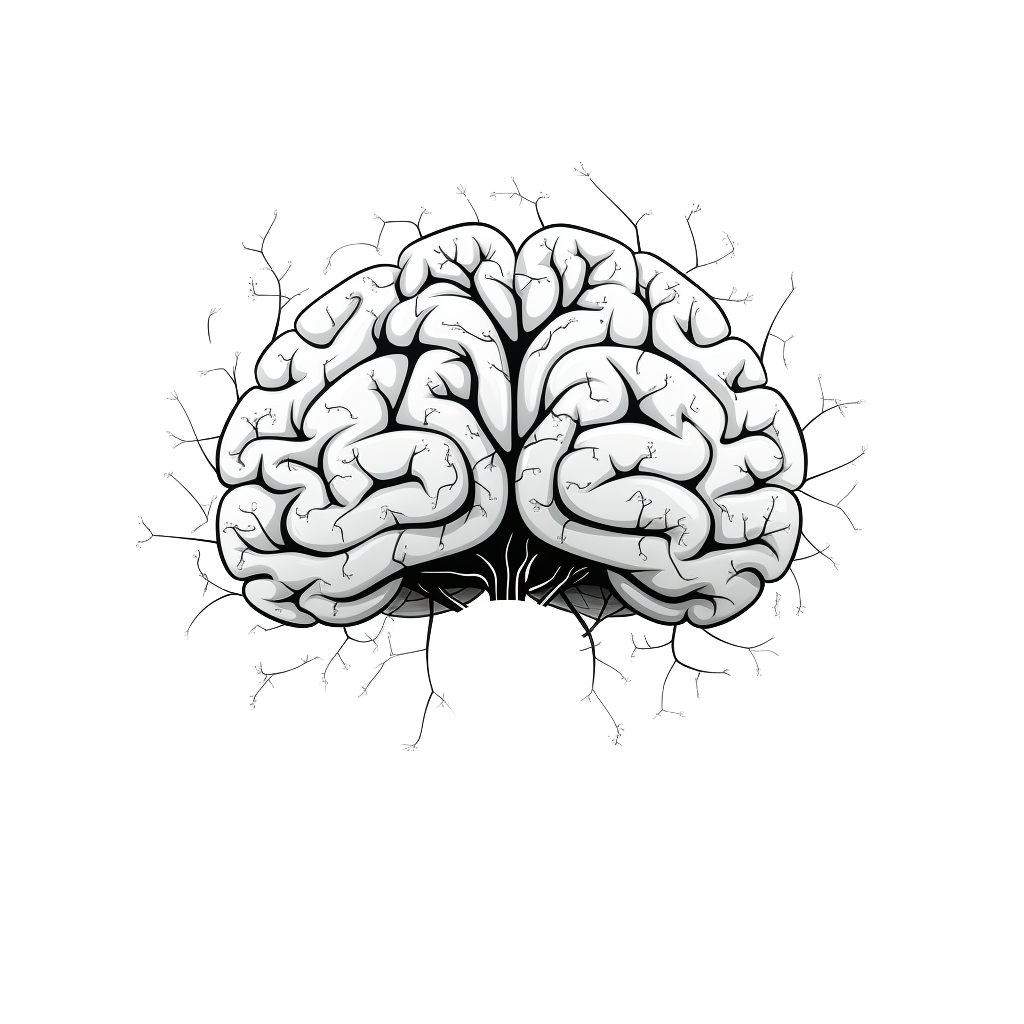
\includegraphics[width=.45\textwidth]{contents/01-introduction/figs/01-fep-brain.png}};
  \node[inner sep=0pt, opacity=0.25] (planet)[left=of center, xshift=3.5mm]{
\includegraphics[width=.45\textwidth]{contents/01-introduction/figs/01-fep-planet.png}};

  \node[box, minimum width=30mm, minimum height=10mm, fill=white](hidden)[left=of center, xshift=-10mm]{Hidden states};
  \node[box, minimum width=30mm, minimum height=10mm, fill=white](model)[right=of center, xshift=10mm]{Internal model};
  \node[box, minimum width=30mm, minimum height=10mm](sensory)[above=of center]{Sensory input};
  \node[box, minimum width=30mm, minimum height=10mm](actions)[below=of center]{Actions};

   \path[line, thick] (hidden) edge[out=90,in=180] node [] {} (sensory);
   \path[line, thick] (sensory) edge[out=0,in=90] node [] {} (model);
   \path[line, thick] (model) edge[out=270,in=0] node [] {} (actions);
   \path[line, thick] (actions) edge[out=180,in=270] node [] {} (hidden);

   \path[line, thick] (model) edge[out=180,in=270] node [] {} (sensory);
   \path[line, thick] (hidden) edge[out=0,in=90] node [] {} (actions);
   \path[line, thick, <->] (sensory) edge[out=270,in=90] node [] {} (actions);

\end{tikzpicture}